% CVPR 2024 Paper Template; see https://github.com/cvpr-org/author-kit

\documentclass[10pt,twocolumn,letterpaper]{article}

%%%%%%%%% PAPER TYPE  - PLEASE UPDATE FOR FINAL VERSION
% \usepackage{cvpr}              % To produce the CAMERA-READY version
\usepackage[review]{cvpr}      % To produce the REVIEW version
% \usepackage[pagenumbers]{cvpr} % To force page numbers, e.g. for an arXiv version
\usepackage{footmisc}
% Import additional packages in the preamble file, before hyperref
%
% --- inline annotations
%
\usepackage[dvipsnames]{xcolor}
\newcommand{\red}[1]{{\color{red}#1}}
\newcommand{\todo}[1]{{\color{red}#1}}
\newcommand{\TODO}[1]{\textbf{\color{red}[TODO: #1]}}
% --- disable by uncommenting  
% \renewcommand{\TODO}[1]{}
% \renewcommand{\todo}[1]{#1}



% It is strongly recommended to use hyperref, especially for the review version.
% hyperref with option pagebackref eases the reviewers' job.
% Please disable hyperref *only* if you encounter grave issues, 
% e.g. with the file validation for the camera-ready version.
%
% If you comment hyperref and then uncomment it, you should delete *.aux before re-running LaTeX.
% (Or just hit 'q' on the first LaTeX run, let it finish, and you should be clear).
\definecolor{cvprblue}{rgb}{0.21,0.49,0.74}
\usepackage[pagebackref,breaklinks,colorlinks,citecolor=cvprblue]{hyperref}
\usepackage{multirow}
%%%%%%%%% PAPER ID  - PLEASE UPDATE
\def\paperID{11499} % *** Enter the Paper ID here
\def\confName{CVPR}
\def\confYear{2024}

%%%%%%%%% TITLE - PLEASE UPDATE
\title{
Active Generation Network of Human Skeleton for Action Recognition
}

%%%%%%%%% AUTHORS - PLEASE UPDATE
\author{Long Liu \footnote{Corresponding author}\\
% Xi'an University of Technology\\
% Xi'an, Shaanxi Province, China\\
{\tt\small liulong@xaut.edu.cn}
% For a paper whose authors are all at the same institution,
% omit the following lines up until the closing ``}''.
% Additional authors and addresses can be added with ``\and'',
% just like the second author.
% To save space, use either the email address or home page, not both
\and
Xin Wang\\
{\tt\small wangxin2168@163.com}
\and
Fangming Li\\
{\tt\small 2220321220@stu.xaut.edu.cn}
\and
Jiayu Chen\\
{\tt\small cjy21123@163.com}
}

\begin{document}
\maketitle
\begin{abstract}
 Current monocular 3D scene reconstruction (3DR) works are either fully-supervised, or not generalizable, or implicit in 3D representation. We propose a novel framework - \textbf{MonoSelfRecon} that for the first time achieves \textbf{explicit 3D mesh} reconstruction for \textbf{generalizable} indoor scenes with monocular RGB views by purely \textbf{self-supervision} on voxel-SDF (signed distance function). MonoSelfRecon follows an Autoencoder-based architecture, decodes voxel-SDF and a generalizable Neural Radiance Field (NeRF), which is used to guide voxel-SDF in self-supervision. We propose novel self-supervised losses, which not only support pure self-supervision, but can be used together with supervised signals to further boost supervised training. Our experiments show that "MonoSelfRecon" trained in pure self-supervision outperforms current best self-supervised indoor depth estimation models and is comparable to 3DR models trained in fully supervision with depth annotations. MonoSelfRecon is not restricted by specific model design, which can be used to any models with voxel-SDF for purely self-supervised manner. %\footnote{Datasets  were  downloaded  and  evaluated  solely  by  the researchers from UC San Diego.}
\end{abstract}    
\section{Introduction} \label{intro}


With the recent development of deep generative models, speech synthesis has seen an extraordinary progress. Among the conventional speech synthesis methods, WaveNets~\cite{oord2016wavenet} were demonstrated to generate high-fidelity audio samples in an autoregressive manner yet suffering from prohibitively expensive computational costs. In contrast, non-autoregressive approaches such as flow-based and GAN-based models~\cite{prenger2019waveglow,jang2021univnet,kong2020hifi,huang2021multi} were also proposed to generate speech audios with satisfactory speed. However, these models were still criticized for other problems, e.g., the limited sample quality or sample diversity \cite{xiao2021tackling}.

In speech synthesis, our goal is mainly two-fold:
\begin{itemize}
    \item High-quality: generating high-quality speech is a challenging problem especially when the sampling rate of an audio is high. It is vital to reconstruct details at different timescales for waveforms of highly variable patterns.
    \item Fast: high generation speed is essential when considering real-time speech synthesis. This poses a challenge for all high-quality neural synthesizers.
\end{itemize}

As a blossoming class of generative models, denoising diffusion probabilistic models (DDPMs)~\cite{ho2020denoising,song2020denoising,lam2022bddm,liu2022pseudo} has emerged to prove its capability to achieve leading performances in both image and audio syntheses~\cite{dhariwal2021diffusion,san2021noise,kong2020diffwave,chen2020wavegrad,lam2022bddm}. However, current development of DDPMs in speech synthesis was hampered by two major challenges:
\begin{itemize}
\item Different from other existing generative models, diffusion models are not trained to directly minimize the difference between the generated audio and the reference audio, but to de-noise a noisy sample given an optimal gradient. This in practice could lead to overly de-noised speech after a large number of sampling steps, in which natural voice characteristics including breathiness and vocal fold closure are removed.
\item While DDPMs inherently are gradient-based models, a guarantee of high sample quality typically comes at a cost of hundreds to thousands of de-noising steps. When reducing the sampling steps, an apparent degradation in quality due to perceivable background noise is observed.
\end{itemize}

In this work, we propose FastDiff, a fast conditional diffusion model for high-quality speech synthesis. To improve audio quality, FastDiff adopts a stack of time-aware location-variable convolutions of diverse receptive field patterns to efficiently model long-term time dependencies with adaptive conditions. To accelerate the inference procedure, FastDiff also includes a noise schedule predictor, which derives a short and effective noise schedule and significantly reduces the de-noising steps. Based on FastDiff, we also introduce an end-to-end phoneme-to-waveform synthesizer FastDiff-TTS, which simplifies the text-to-speech generation pipeline and does not require intermediate features or specialized loss functions to enjoy low inference latency.

Experimental results demonstrated that FastDiff achieved a higher MOS score than the best publicly available models and outperformed the strong WaveNet vocoder (MOS: 4.28 vs. 4.20). FastDiff further enjoys an effective sampling process and only needs 4 iterations to synthesize high-fidelity speech, 58x faster than real-time on a V100 GPU without engineered kernels. To the best of our knowledge, FastDiff is the first diffusion model with a sampling speed comparable to previous  for the first time applicable to interactive, real-world speech synthesis applications at a low computational cost. FastDiff-TTS successfully simplify the text-to-speech generation pipeline and outperform competing architectures.

\section{Related work}

\textbf{Generative Adversarial Networks. }
Generative Adversarial Networks (GAN) is a generative models which is trained by adversarial learning. 
In the early days, unconditional GAN \cite{karras2019style,karras2020analyzing} recovered images from random noise. Developed to the present, conditional GAN \cite{pan2023drag} utilizes text and images for guidance to generate images. GAN has performed strongly on tasks of generating static data such as image generation \cite{karras2019style, karras2020analyzing}, image editing \cite{vinker2021image, patashnik2021styleclip}, and image translation \cite{shao2021spatchgan}.
The generation of dynamic data, such as videos and action sequences, has also been studied. Carl et al. \cite{vondrick2016generating} proposed a video generation network with a spatial-temporal two-stream convolutional architecture based on DCGAN \cite{radford2015unsupervised}. This work is the first application of GAN to video generation. 
TGAN \cite{saito2017temporal} followed, which first generates a set of latent vectors from noise vectors, then generates pictures and synthesizes videos separately.
RNN-GAN \cite{mogren2016c} is based on the temporal modeling capability of RNNs to predict video from a single frame. It has a more robust motion prediction capability compared to the work of Carl et al. However, these impressive results are mainly attributed to the support of many training samples. With limited data, GANs are prone to overfitting, leading to a lack of diversity in the generated data. 

% \textbf{Few-shot Generation. }

\textbf{Motion Style Transfer. }
Image Style Transfer \cite{gatys2016image, saito2020coco} combines style and content features from two images to form a new image. Motion Style Transfer refers to Image Style Transfer to form a new action by transferring one action's style features to another that contains only content features. Early motion style transfer was done by manually defining style features and inferring them through machine learning \cite{xia2015realtime, yumer2016spectral}. This method is effective only for the actions in the training data with limited scope of usefulness. 
Deep learning-based methods have greatly improved the quality and application of motion style transfer. Both Holden et al. \cite{2016A} and Du et al. \cite{du2019stylistic} applied the Gram matrix method to convey motion styles through the distribution of actions in the hidden space. These methods are time-consuming and have limited the quality of action generation for relatively significant motion differences.
Recently, Aberman et al. \cite{aberman2020unpaired} proposed a motion transfer network that combines GAN and AdaIN. 
The method can learn from unpaired data with different styles to migrate model unseen actions. 
Park et al. \cite{ParkSoomin2021Diverse} used a spatio-temporal graph convolutional network to model actions. The method adds random noise in the decoder to enhance action diversity. 
Jang et al. \cite{jang2022motion} proposed a novel motion style transfer network called Motion Puzzle. 
Motion Puzzle divides the human skeleton into five parts, allowing flexible control over the migration of specified parts during generation. This approach is effective for single-action generation tasks.
However, it is usually time-consuming to control parts for generation when generating many actions. In addition, Motion Puzzle's target motion encoder is connected to the decoder at multiple scales, which may constrain the diversity of action.

\textbf{Active Learning. }
Existing active learning methods are categorized into pool-based and synthetic methods \cite{gal2016dropout,beluch2018power,gorriz2017cost,yang2017suggestive,nguyen2004active}. Pool-based methods use different sampling strategies to determine how to select the most informative samples, with uncertainty sampling methods being the most common.
Ebrahimi et al. \cite{ebrahimi2019uncertainty} used a Bayesian neural network for uncertainty evaluation. Gal \cite{gal2016dropout} and Gharamani \cite{gal2017deep} also showed the relationship between uncertainty and dropout to estimate uncertainty in neural network prediction.
Pool-based methods select samples conditional on a large amount of unlabeled data. In the case of scarcity of data, synthetic methods are more suitable than pool-based methods. Synthetic methods use a generative model to generate samples, then sample based on the uncertainty of the model.
The work of Zhu et al.  \cite{zhu2017generative}, Mahapatra et al.  \cite{mahapatra2018efficient}, and Mayer et al. \cite{mayer2020adversarial} uses GAN to generate a sample and then query using the uncertainty principle. Our work uses this same strategy to guide human action generation using the amount of sample information.

%body poses $\{\bm{\theta}^{(t)}\}$, node residual translations $\{\Delta\bm{n}_i^{(t)}\}$ and dynamic detail embeddings $\{\bm{e}_i^{(t)}}\}$.

\section{Method}
\label{sec:method}
Having elaborated on the proposed representation, we turn to network learning in this section. 
Specifically, we need to determine the aforementioned variables alongside with the weights of the radiance networks for a training image sequence $\bm{I}_t, t=1, 2,..., T$. The images can be captured from a multi-view system or a monocular one. In order to synthesize images for new poses, we also have to compute the node residual translations and the dynamic detail embeddings corresponding to those poses. 
We assume access to the body poses of the training images (\textit{i.e.}, $\bm{\theta}^{(t)}, t=1, 2, ..., T$), which can be estimated using marker-less MoCap tools such as \cite{easymocap,lightcap2021}. The node residual translations and the detail embeddings are referred to as ``node-related variables" in the following context. 



% Having elaborated on the proposed representation, we turn to network learning in this section. 
% Specifically, we need to determine the aforementioned variables (i.e., body poses, node residual translation and dynamic detail embeddings) as well as the weights of the radiance networks for a training sequence $\bm{I}_t, t=1, 2,..., T$. In order to synthesize images for new poses, we also have to compute the node residual translations and the dynamic detail embeddings corresponding to those specific poses. In this work, we assume access to the body poses of the training images, which can be easily obtained using existing marker-less MoCap algorithm such as \cite{easymocap}. 

% In Sec.~\ref{sec:method:arch} and ~\ref{sec:method:loss}, we discuss how to determine the aforementioned variables as well as the weights of the radiance networks for a training image sequence $\bm{I}_t, t=1, 2,..., T$. In order to synthesize images for new poses after training, we also need to compute the node residual translations and the dynamic detail embeddings corresponding to those specific poses (Sec.~\ref{sec:method:animation}). In this work, we assume access to the body poses of the training images, which can be easily obtained using existing marker-less MoCap algorithm such as \cite{easymocap}. 


\subsection{Network Architecture}
\label{sec:method:arch}
To obtain the node-related variables for the training frames and ensure generalization during animation, we design a simple conditional variational auto-encoders (cVAE)~\cite{Sohn2015cvae} as an auxiliary network for each node. 
% Naive optimization during network training make it difficult to generate the variables for new poses after training, while directly regressing them from pose condition leads to one-to-many problem as the similar poses can lead to different cloth wrinkles in reality. 
% A naive solution to obtain the node residual translation and dynamic detail embeddings is using optimization during network training (i.e., auto-decoding~\cite{park2019deepsdf}). However, this will make it difficult to generate the variables for new poses during training. What's worse, naive optimization cannot guarantee information distanglement, which further hinders generalization~\cite{timur2021driving_signal}. 
% Drawing inspiration from \cite{timur2021driving_signal}, we design a simple conditional variational auto-encoder ~\cite{Sohn2015cvae} for each node as an auxiliary network. Each cVAE consists of an encoder and a decoder, both implemented with MLPs. 
Each auxiliary network consists of an encoder and a decoder, both implemented with tiny MLPs. 
Following the practice of SCANimate~\cite{Saito:SCANimate:2021}, the condition variable of this cVAE is the pose vector multiplied by the skinning weight and an attention map:
\begin{equation}
    \bm{\theta}^{(t)}_i = (\bm{\mathrm{W}}\cdot \bm{\omega}_i) \circ \bm{\theta}^{(t)}, 
\end{equation}
where $\bm{\mathrm{W}}$ is the weight map that converts the skinning weights into pose attention weights as in \cite{Saito:SCANimate:2021} and $\circ$ denotes element-wise product. 
During training, the encoder takes the time stamp $t$ as input and $\bm{\theta}^{(t)}_i$ as condition, and produces parameters of a Gaussian distribution, from which a latent code $\bm{z}_i^{(t)}$ is sampled:
\begin{equation}
\label{eqn:latent_sample}
    \bm{\mu}_i^{(t)}, \bm{\sigma}_i^{(t)} \gets \mathcal{E}(t, \bm{\theta}_i^{(t)}), \ \bm{z}_i^{(t)} \sim \mathcal{N}(\bm{\mu}_i^{(t)}, \bm{\sigma}_i^{(t)}), 
\end{equation}
% In practice we augment the time stamp with periodic encoding~\cite{mildenhall2020nerf}. 
Conditioned on the body pose, the latent code is then decoded into the node residual translation and the dynamic detail embedding:
\begin{equation}
    \Delta\bm{n}_i^{(t)},  \bm{e}_i^{(t)} \gets \mathcal{D}(\bm{z}_i^{(t)}, \bm{\theta}_i^{(t)}), 
\end{equation}
which are later used in Eqn.~(\ref{eqn:reprez:local_coord}) and  Eqn.~(\ref{eqn:reprez:feat_fusion}), respectively. 

In this network, the time instant is used to distinguish similar poses at different time instants, thereby avoiding the one-to-many mapping issue. With the KL-divergence loss in cVAE, there is a preference to let the decoder to mainly rely on the pose condition for prediction, and the time input only provides information necessary for good reconstruction.  
In our implementation, we augment the time stamp and the coordinates with Fourier encoding before feeding them into MLPs~\cite{mildenhall2020nerf} . Fig.~\ref{fig:network} illustrates the data flow in our network during training. Once the training is done, we can render the model for either training frames or novel poses. To render the training sequence, we use the full network and set $\bm{z}_i^{(t)} = \bm{\mu}_i^{(t)}$ in Eqn.~(\ref{eqn:latent_sample}) to eliminate randomness. When unseen poses are given, the encoder half of the cVAE will be omitted and $\bm{z}_i^{(t)}$ will be set to zeros. 


\subsection{Training Loss}
\label{sec:method:loss}
Our network can be trained in an end-to-end manner. 
The training loss is composed of four components, including a reconstruction loss, a node translation regularization, an embedding regularization, and a KL-divergence loss:
\begin{equation}
     \mathcal{L} = \lambda_{rec}\mathcal{L}_{rec} + \lambda_{trans}\mathcal{L}_{trans} + \lambda_{ebd}\mathcal{L}_{ebd} + \lambda_{KL}\mathcal{L}_{KL}.
\end{equation}
Below we discuss them in details. For ease of notation, we drop the superscript ${}^{(t)}$ of all variables in this subsection. 

\textbf{Reconstruction Loss} $\mathcal{L}_{rec}$ measures the mean squared error between the rendered and true pixel colors:
\begin{equation}
    \mathcal{L}_{rec} = \sum_{\bm{r}\in\mathcal{R}} \left\Vert \bm{C}\left(\bm{r} | \bm{\theta}, \{\Delta\bm{n}_i\}, \{\bm{e}_i\}\right) - \hat{\bm{C}}_{\bm{r}}  \right\Vert_2^2, 
\end{equation}
where $\mathcal{R}$ is the set of rays in each batch, $\hat{\bm{C}}_{\bm{r}}$ is the ground-truth pixel color, $\bm{C}(\cdot | \bm{\theta}, \{\Delta\bm{n}_i\}, \{\bm{e}_i\})$ is the volume rendering function with the representation defined in Sec.~\ref{sec:overview}. 

\textbf{Node Translation Regularization} $\mathcal{L}_{trans}$ simply constrains the position change of each nodes in order to stabilize training: 
\begin{equation}
    \mathcal{L}_{trans} = \sum_i \Vert \Delta\bm{n}_i \Vert_2^2. 
\end{equation}

\textbf{Embedding Regularization} $\mathcal{L}_{ebd}$ penalize large magnitudes of the dynamic detail embeddings: 
\begin{equation}
    \mathcal{L}_{ebd} = \sum_i \Vert \bm{e}_i \Vert_2^2. 
\end{equation}
% It is inspired by \cite{park2019deepsdf} and 
A similar loss is also used in \cite{park2019deepsdf}; here we utilize it to encourage the embeddings to encode only the information that cannot be represented by node position. 
%and can push the latent embeddings to become uninformative. 
% Through tuning the value of $\lambda_{trans}$ and $\lambda_{ebd}$, we can encourage the embeddings to encode only the information that cannot be represented by node position. 

\textbf{KL-divergence Loss} $\mathcal{L}_{KL}$ is a standard VAE KL-divergence penalty~\cite{kingma2014vae}:
\begin{equation}
    \mathcal{L}_{KL} = \sum_i \mathrm{KL}\left( \mathcal{N}(\bm{\mu}_i, \bm{\sigma}_i) \ \Vert\  \mathcal{N}(\bm{0}, \bm{\mathrm{I}})\right).
\end{equation}

% \subsection{New Pose Synthesis}
% \label{sec:method:animation}


\begin{figure}
    \centering
    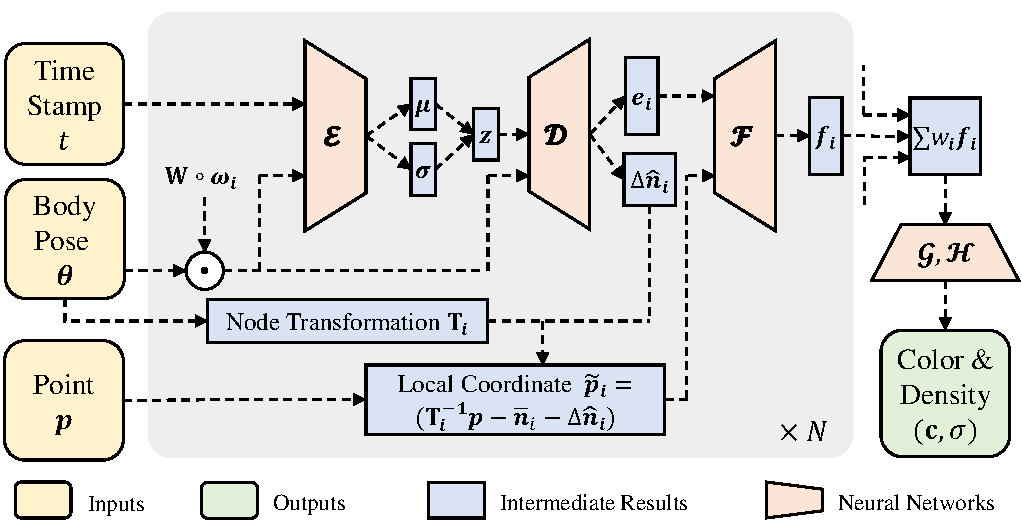
\includegraphics[width=1.0\linewidth]{network}
    \caption{\textbf{Illustration of the data flow in our network.} The time stamp and body pose feature are first passed through the cVAEs, which produces the node residual translations and dynamic detail embeddings of the local radiance fields. For a point in the posed space, we calculate its local coordinate in each local field, and then query its feature. Finally, all features are blended and decoded into the color and density values.   }
    \label{fig:network}
\end{figure}





\noindent\textbf{Implementation Details}
The local radiance networks and cVAEs in our architecture are implemented with parallel tiny MLPs in the form of group 1D convolution.
To accelerate training and inference, we exploit the fact that, for any point in the posed space, only a small portion of nodes have influence on its color and density value. 
We use Adam optimizer to train our models. Training the whole models takes about 25 hours on one NVIDIA 3090 GPU with 500k iterations, while rendering an color image with resolution of $512\times 512$ typically takes 5 seconds on one NVIDIA 3080TI GPU. Please refer to the \textit{Supp.Mat.} for more details. 



\section{Experiments}

We conducted various experiments to prove the effectiveness of the present method. 
Firstly, we qualitatively measure the results of our method on seen and unseen data, including action visualization and data downscaling visualization. 
Secondly, the generation quality and accuracy of action recognition were quantitatively measured for the six categories of target actions.
Finally, we performed comparison experiments with previous methods and ablation experiments with a special training loss term.
In addition, we train the ST-GCN using generated and real data, respectively, and test the accuracy of the same real data, thus evaluating the degree of approximation between the generated and real data. 

\subsection{Action Generation}

\textbf{Qualitative evaluation. }
Figure. \ref{fig:4} shows the generated seen actions. 
(a) and (b) are the “Reach into Pocket” and “Hopping” actions generated with reference to “Brush Hair”, respectively, the former being a hand motion and the latter a whole-body motion. 
(c) and (d) are the “Put Palms Together” and “Bow” actions generated with reference to “Hopping”, respectively. 
All the above actions preserve the source action $\textbf{M}_{src}$ category features and target action $\textbf{M}_{tgt}$ morphological features. 
Compared with Motion Puzzle, this method can generate hand, upper limb, and whole body actions without specifying body parts. 
Meanwhile, the temporal consistency of the actions is guaranteed, e.g., the real and generated “Hopping” are jumping at the same time in (b), and the bending tendency of the generated and real actions are consistent in (d). 

\begin{figure*}[htpb]
  \centering
   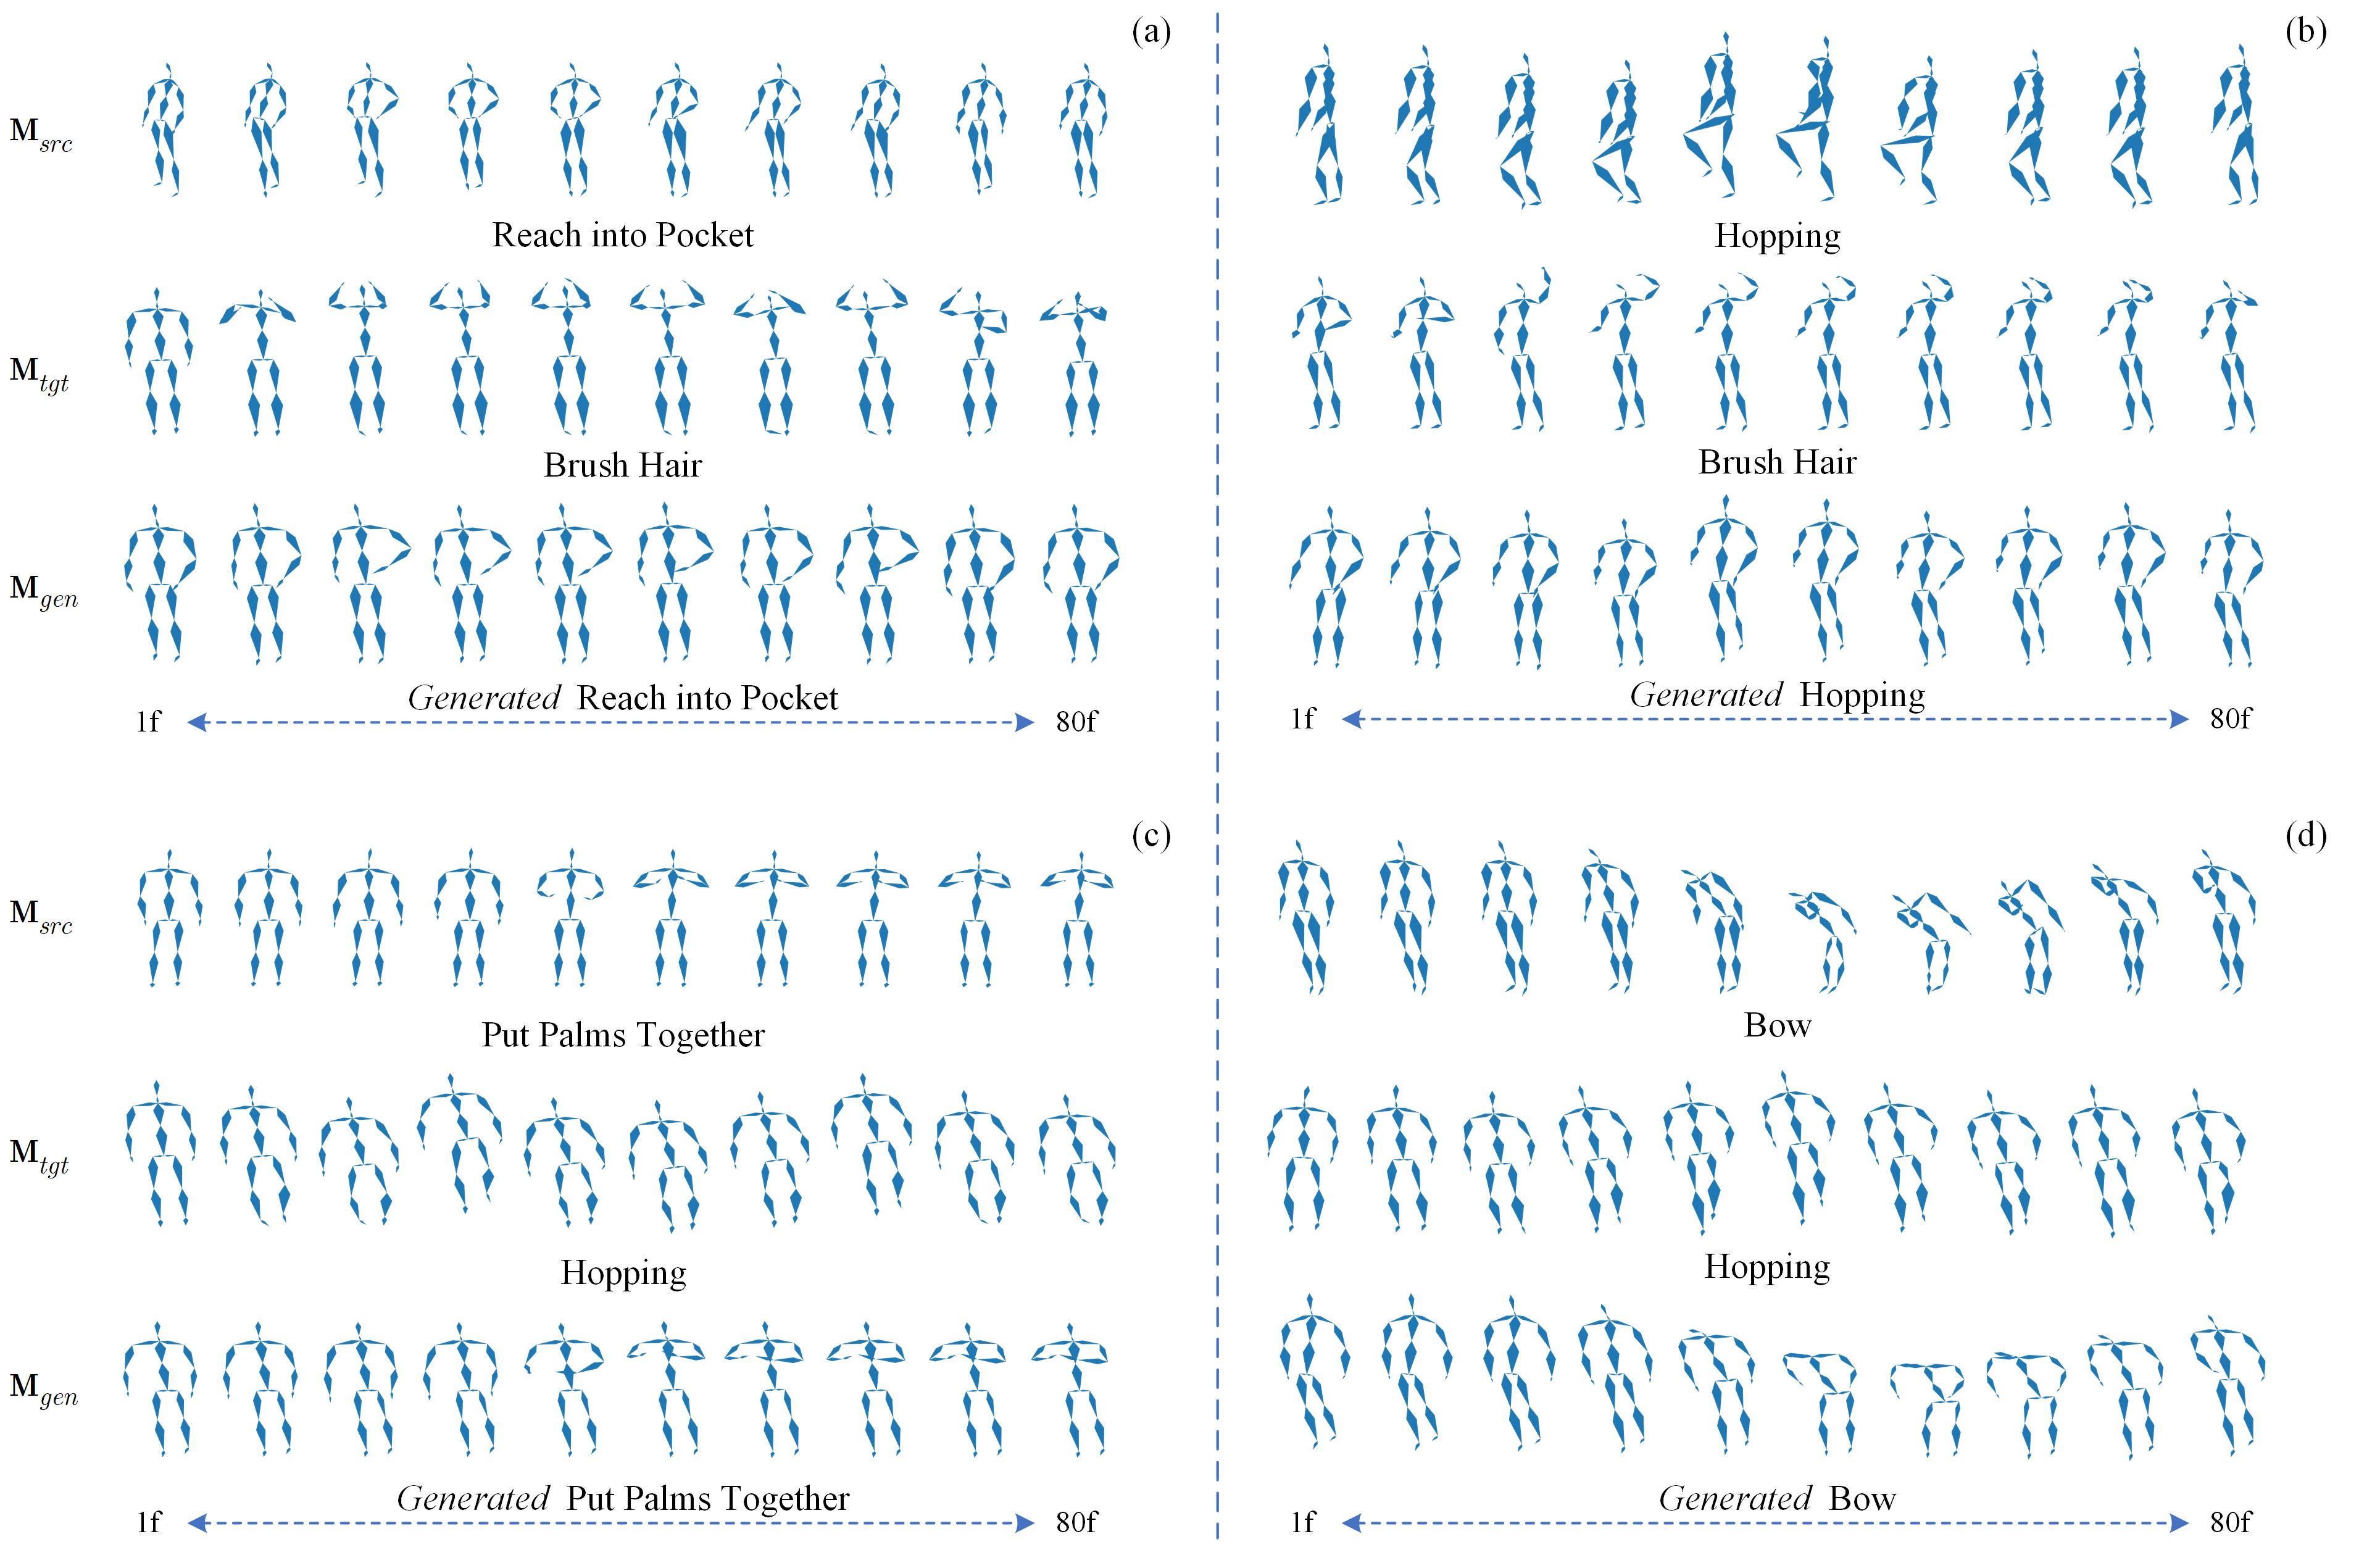
\includegraphics[width=0.75\linewidth]{figures/Fig4.jpg}

   \caption{Results generated by MGN on seen actions. (a) “Reach into Pocket”. (b) “Hopping”. (c) “Put Palms Together”. (d) “Bow”.}
   \label{fig:4}
\end{figure*}

Figure. \ref{fig:5} shows the generated unseen motions. 
It contains three cases: only the source action is unseen, only the target action is unseen, and both are unseen to thoroughly verify the transfer effect of unseen actions. 
In (a) and (f), the source action $\textbf{M}_{src}$  (“Drink Water” and “Jump Up”) is unseen, while the target action $\textbf{M}_{tgt}$  (“Kicking Something”) is seen. The generated action $\textbf{M}_{gen}$ can keep the category information of the source action. 
In (c) and (d), $\textbf{M}_{src}$  is seen, and $\textbf{M}_{tgt}$ is unseen. In $\textbf{M}_{gen}$, the morphological features of $\textbf{M}_{tgt}$ are transferred, and the “Kicking Something” action of $\textbf{M}_{src}$ is retained. 
Both source and target actions are unseen in (b) and (e). $\textbf{M}_{gen}$ shows that the model is still able to extract the category information of $\textbf{M}_{src}$ and the morphology information of $\textbf{M}_{tgt}$ to form a new action.
From the generated actions in Figure. \ref{fig:5}, our model can still generate high-quality actions that are unseen for the model.

\begin{figure*}[htpb]
  \centering
   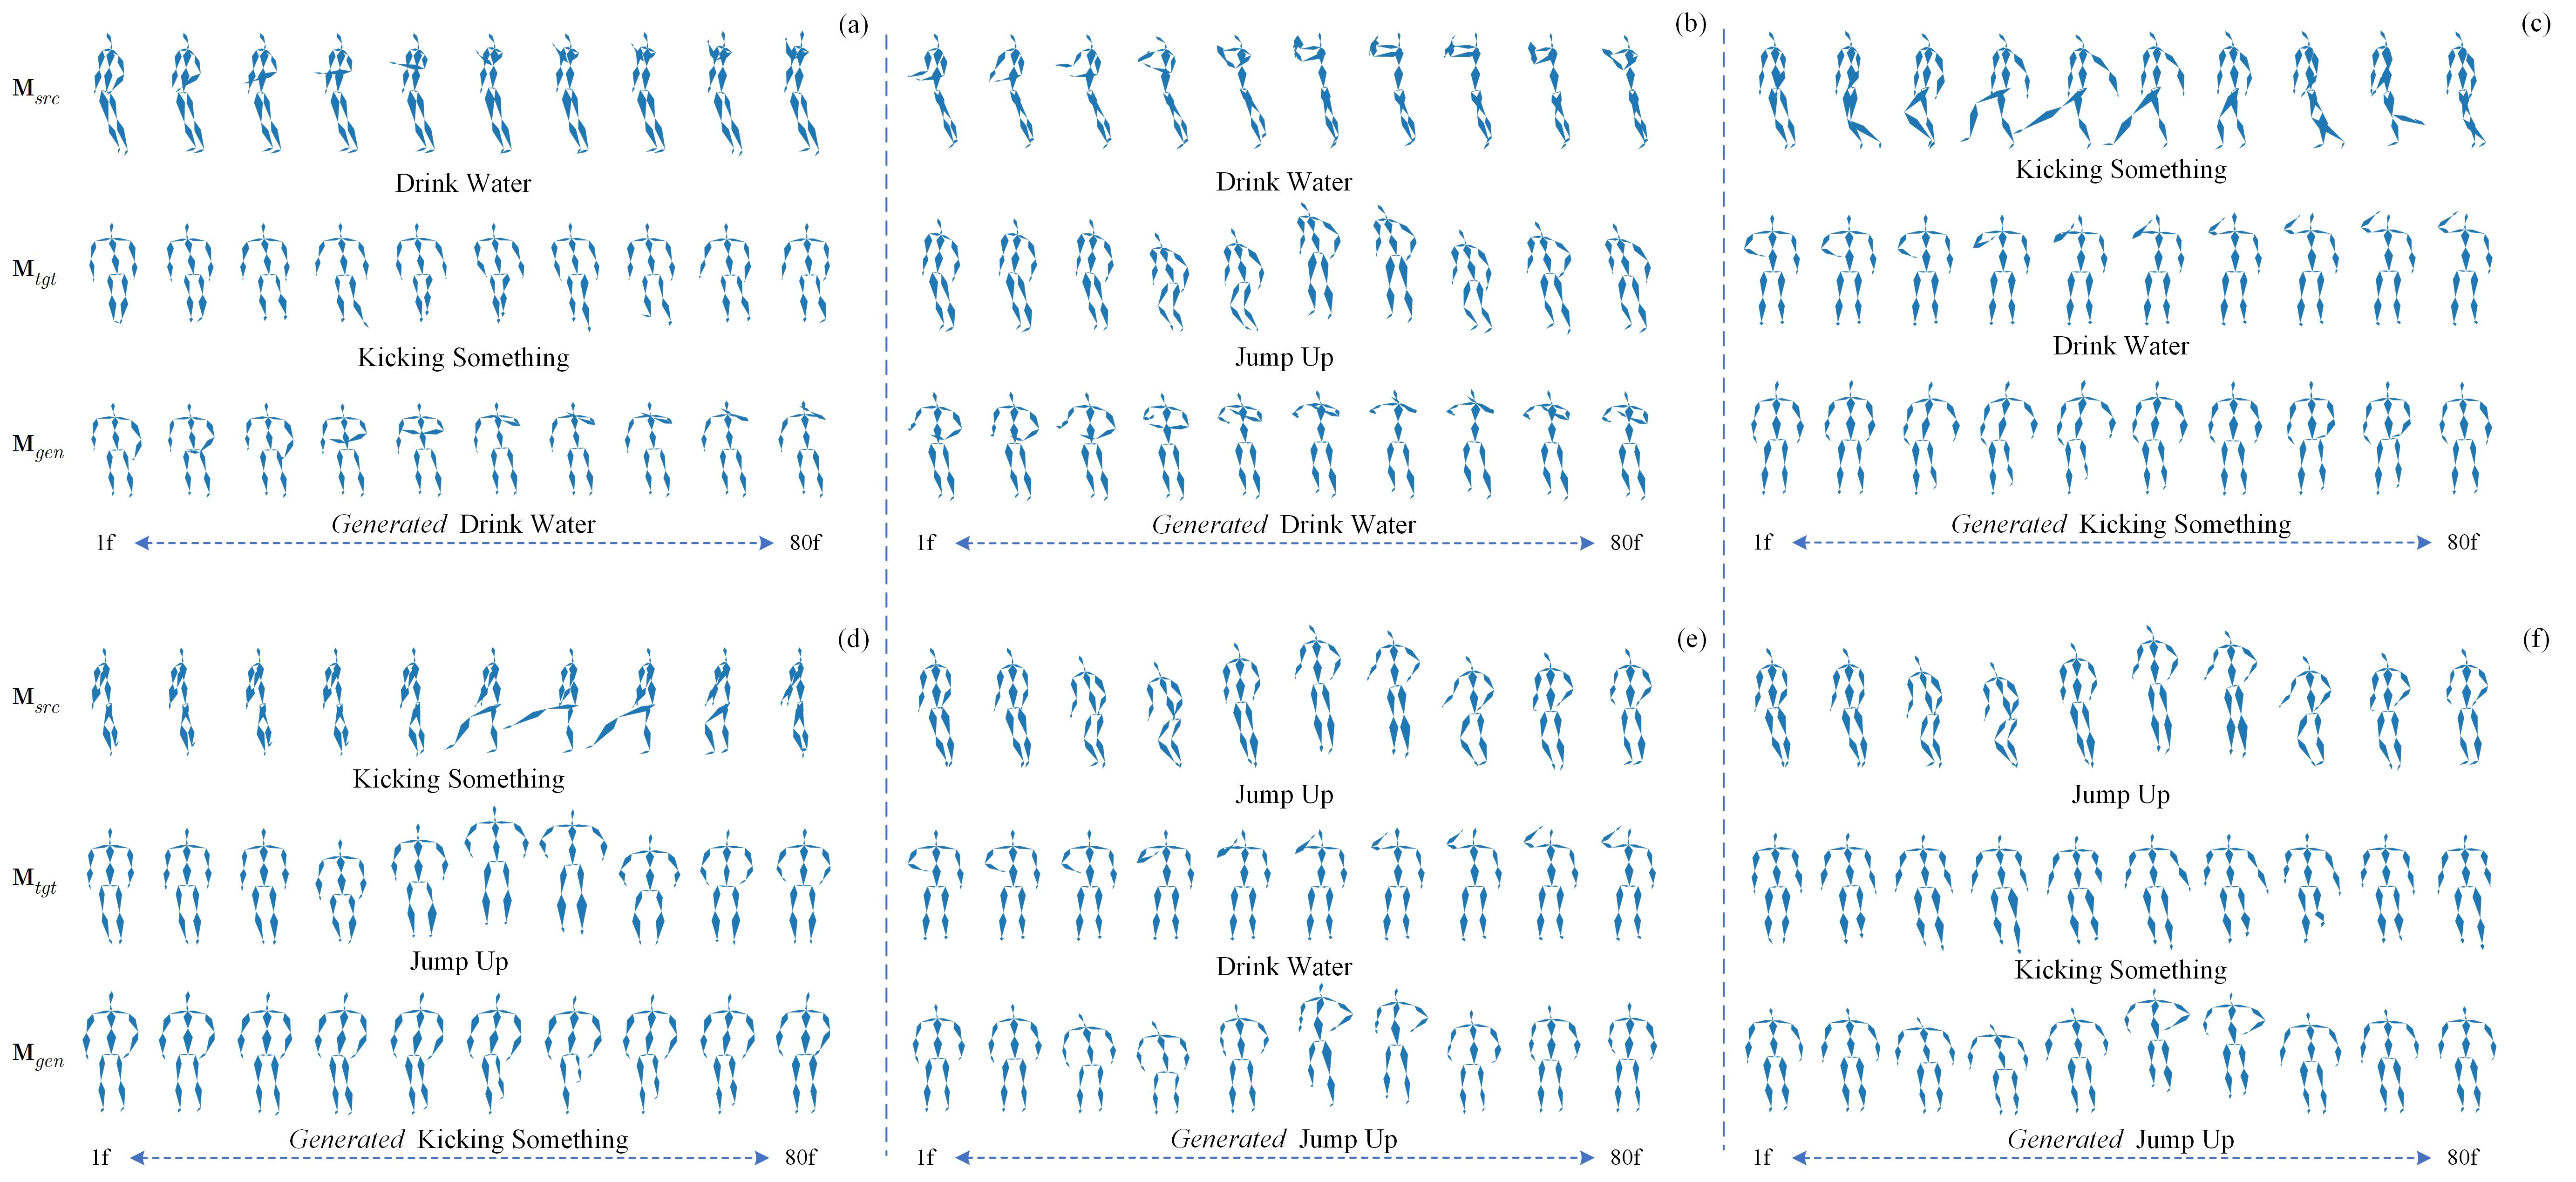
\includegraphics[width=\linewidth]{figures/Fig5.jpg}

   \caption{Results generated by MGN on unseen actions. (a) and (b) are  “Drink water” (Unseen). (c) and (d) are “Kicking Something” (Seen). (e) and (f) are “Jump Up” (Unseen).}
   \label{fig:5}
\end{figure*}

In order to verify the approximation between the generated data and the real data, t-SNE was used to visualize the action data. 
Figure. \ref{fig:3} shows the data distribution after dimensionality reduction using t-SNE. The black and red samples in the figure are the source actions, where red is a random sample in black. Cyan samples are the target actions, while green are the generated samples. The six figures show that the distribution of new actions generated using only one source action is similar to the distribution of source actions. The results show that our generated data can replace the original data. 

\begin{figure*}[htpb]
  \centering
   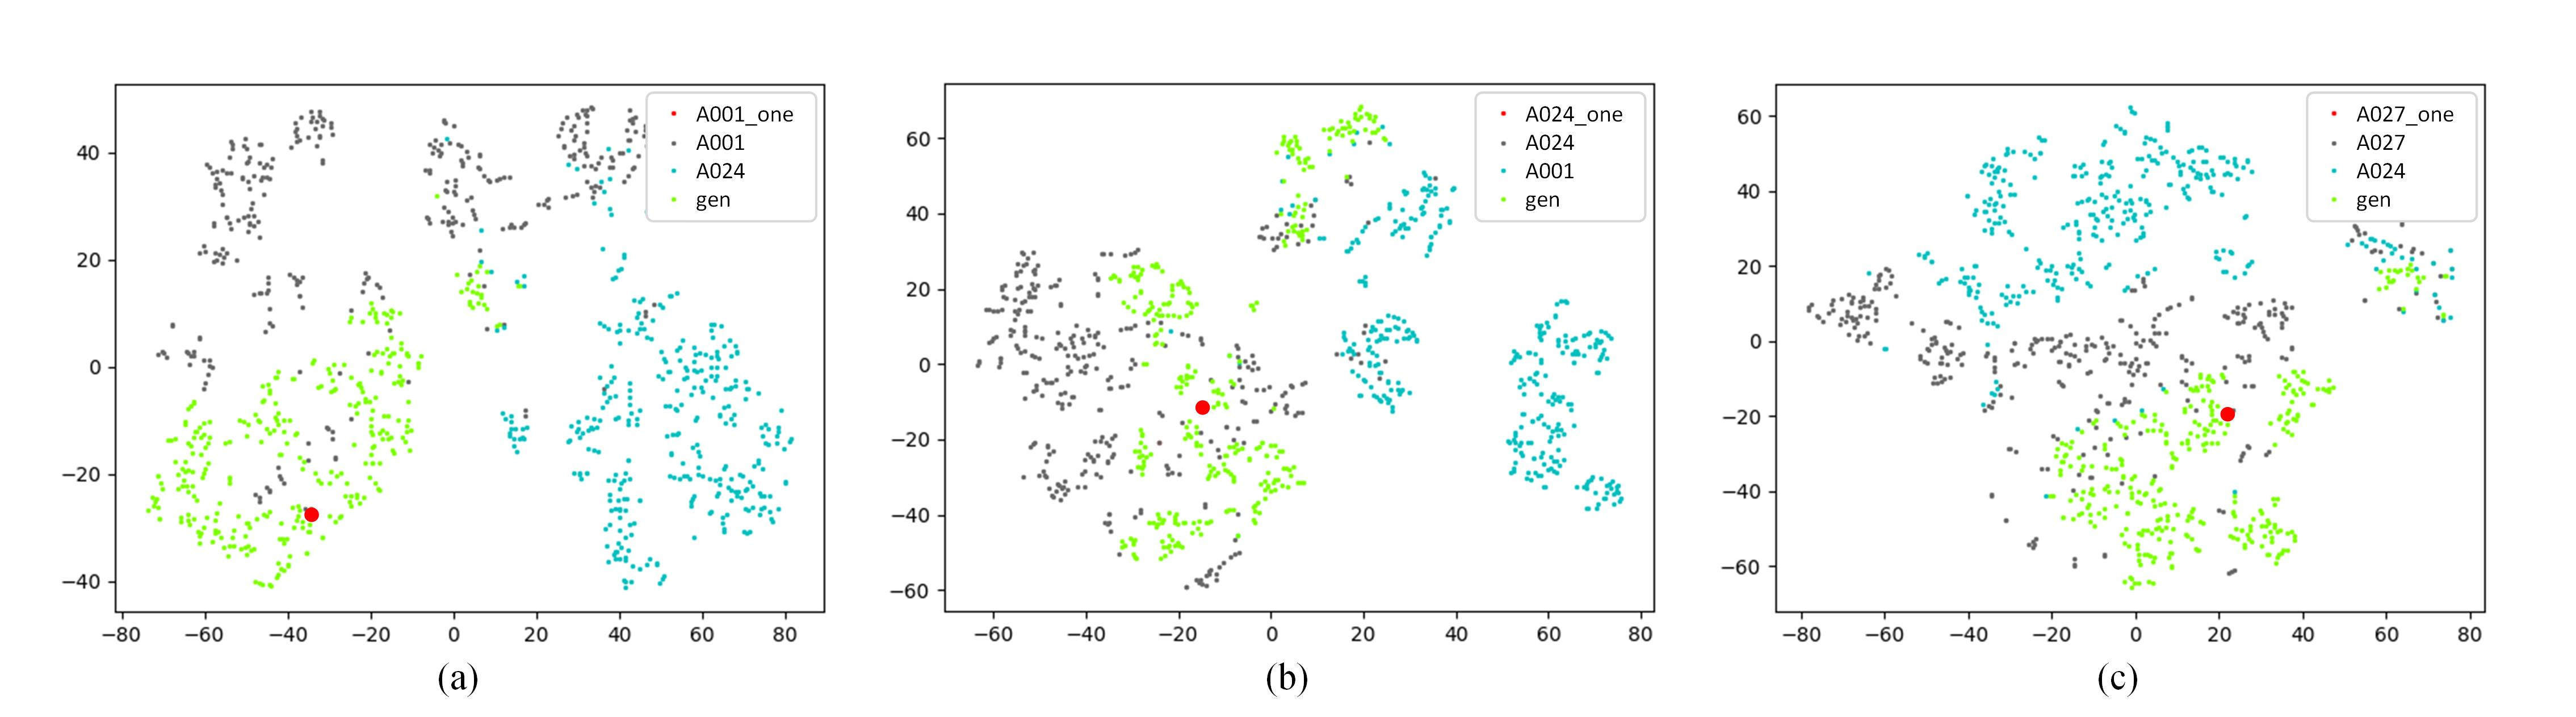
\includegraphics[width=0.8\linewidth]{figures/Fig3.jpg}

   \caption{Action data is projected into 2D space using t-SNE, where black is the source action, red is a sample of black, cyan is the target action, and green is some new action generated using a sample of red and some cyan. The green sample and the black sample are very close to each other in space, which indicates that the generated actions conform to some extent to the distribution of the source actions.}
   \label{fig:3}
\end{figure*}

\textbf{Quantitative evaluation. }
We quantitatively measured the quality of generation and accuracy of action recognition on seen and unseen data. 
Specifically, we use two metrics: Fréchet Motion Distance (FMD) and Accuracy (Acc). 
We compute FMD and Acc on the action set based on all possible combinations of source and target actions generated by the MGN.

The FMD measures the similarity between the feature vectors of real and generated actions, similar to the Fréchet Inception Distance (FID). 
The action classifier is trained by the ST-GCN method, and feature vectors are obtained after the maximum pooling layer to compute the FMD of generated and real actions. 
A lower FMD means a higher quality of action.

% As described in Sec. \ref{sec:Dataset}, 
We complete the experimental evaluation using the action sets $\mathcal{M}_{full}$, $\mathcal{M}_{seen}$, and $\mathcal{M}_{unseen}$. 
The $\mathcal{M}_{seen}$ contains six categories of seen actions data: “Brush Teeth”, “Pick up”, “Reading”, “Take off a Hat”, “Kicking Something”, and “Sneeze”, for 3996 samples. 
The $\mathcal{M}_{unseen}$ contains six categories of unseen actions data: “Drink Water”, “Throw”, “Sit Down”, “Clapping”, “Jump up”, and “Bow”, for 3992 samples.
Table \ref{tab:1} shows that the Acc of the generated actions all exceeded 90\%. 
The highest of these is 95.39\%, with an average of 92.18\% under the seen actions data. 
The highest of these is 97.20\%, with an average of 94.42\% under the unseen actions data. 
The mean values of FMD in both cases are 2.11 and 2.67, respectively. This shows that our generated actions are high-quality and can be well recognized by the action classifier. 

\begin{table}
  \centering
  % \begin{tabular}{@{}lc@{}}
  \resizebox{1\columnwidth}{!}{
  \begin{tabular}{cccccccc}
    \toprule
    \multirow{2}*{}&\multirow{2}*{Metric}&\multicolumn{6}{c}{Target motion}\\
\cline{3-8}
    &  &  A0&  A1&  A2&  A3&  A4& A5\\
    \midrule
    \multirow{2}*{Seen}& Acc(\%)&  91.10&  90.12&  94.63&  92.29&  95.39& 89.54\\  
    & FMD &  2.19&  2.00&  1.95&  2.02&  2.18& 2.31\\ 
    \multirow{2}*{Unseen}& Acc(\%)&  97.20&  96.45&  89.62&  90.78&  96.77& 95.72\\
    & FMD &  3.21&  2.49&  2.53&  3.11&  2.30& 2.35\\
    \bottomrule
  \end{tabular}}
  \caption{Quantitative evaluation. We calculated FMD and Acc using $\mathcal{M}_{full}$, $\mathcal{M}_{seen}$, and $\mathcal{M}_{unseen}$. $\mathcal{M}_{full}$ contains six categories of action: “Brush Hair”, “Writing”, “Put on a Shoe”, “Take off Glasses”, “Hopping”, and “Shake Head”. For representation simplicity, we numbered the six categories of target action as A0, A1, A2, A3, A4, and A5.}
  \label{tab:1}
\end{table}

\subsection{Action Recognition}
\label{sec:motion recognition}

Generating compelling and high-quality data is significant for action recognition tasks when specific action categories are scarce. 
In order to measure the degree of similarity between generated and real data fully, an action recognition model is trained using generated and real actions, respectively. 

We divided the actions in $\mathcal{M}_{unseen}$ into a training set $\mathcal{M}_{\hat{train}}$ and a test set $\mathcal{M}_{\hat{test}}$. An action recognition model (ST-GCN) is trained using $\mathcal{M}_{\hat{train}}$ and tested on $\mathcal{M}_{\hat{test}}$. As shown in the Table \ref{tab:2}, the top-1 accuracy is 91.80\%.  
We sample one-shot and few-shot (1\%, 5\%, and 10\%) from $\mathcal{M}_{\hat{train}}$ for action generation. 
Subsequently, the generated and sampled actions are concatenated into a new train set to train and test the ST-GCN. 
As shown in Table \ref{tab:2}, the top-1 accuracy is highest at 91.62\% when sampling 10\%, which is only 0.18\% lower than that of $\mathcal{M}_{\hat{train}}$. When sampling 1\% and 5\%, the top-1 accuracy is still high, close to 90\%. 
However, the top-1 accuracy is lower when sampling one, with a maximum of only 62.84\%. 
This result is expected because when sampling a single sample, the generative model is very limited to learning the source data distribution, leading to a large deviation of the generated data distribution from the original complete data distribution. 

\begin{table}
  \centering
  % \begin{tabular}{@{}lc@{}}
  \resizebox{1\columnwidth}{!}{
  \begin{tabular}{cccccc}
    \toprule
    \multirow{2}*{Target motion}&\multirow{2}*{OneShot(\%)}& \multicolumn{3}{c}{FewShot(\%)} & \multirow{2}*{$\mathcal{M}_{\hat{train}}$(\%)}\\ \cline{3-5} 
        && 1\% & 5\% & 10\% &\\
    \midrule
    A0 & 62.84 & 84.09 & 88.34 & 91.62 & \multirow{6}*{91.80} \\ 
    A1 & 53.31& 79.54 & 89.74 & 90.04 &  \\  
    A2 & 57.62 &  78.14& 89.01 & 91.32 & \\ 
    A3 & 57.07& 81.30& 89.25 & 91.44 & \\
    A4 & 45.96& 82.33 & 88.16& 91.14 & \\
    A5 & 61.57 & 83.49 & 88.46 & 91.01 & \\
    \bottomrule
  \end{tabular}}
  \caption{Top-1 accuracy comparison. Sampling one-shot and few-shot (1\%, 5\%, and 10\%) from $\mathcal{M}_{\hat{train}}$ for action generation. The generated and sampled actions are concatenated into a new train set to train and test the ST-GCN. }
  \label{tab:2}
\end{table}

\subsection{Ablation Study and Comparison with Prior Work}

We conduct an ablation study of the loss term and a comparison with other methods to verify the validity of the loss term in the model and the state-of-the-art of our method. 
Specifically, we quantitatively measure the generation quality and Accuracy of the five generative models: 
$[$Aberman et al. 2020$]$, 
$[$Jang et al. 2022$]$, 
MGN($\mathcal{L}_{rec}+\mathcal{L}_{cyc}$), 
MGN($\mathcal{L}_{rec}+\mathcal{L}_{cyc}+\mathcal{L}_{trip}$), and AGN (Table. \ref{tab:3}).
Where MGN($\mathcal{L}_{rec}+\mathcal{L}_{cyc}+\mathcal{L}_{trip}$) is a part of AGN. Therefore, the FMD is both 2.67. 
Due to the effect of UMN, the recognition accuracy of AGN is 4.76\% higher than the former, which is 87.42\% and 92.18\%, respectively. 
The FMD and Accuracy are 2.90 and 83.43\% for the MGN without $\mathcal{L}_{trip}$, proving that our design of $\mathcal{L}_{trip}$ is effective in generative networks. The method of Aberman et al. measures the FMD to be 21.36 and the Accuracy to be 51.34\%. Motion Puzzle measured an FMD of 9.42 and an Accuracy of 67.63\%.
In comparison, our method is competitive.

\begin{table}
  \centering
  % \begin{tabular}{@{}lc@{}}
  \resizebox{1\columnwidth}{!}{
  \begin{tabular}{lcc}
    \toprule
    Methods&FMD$\downarrow$&Acc(\%)$\uparrow$ \\
    \midrule
    $[$Aberman et al. 2020$]$& 21.36 $\pm$ 2.37& 51.34 $\pm$ 1.92\\
    $[$Jang et al. 2022$]$& 9.42 $\pm$ 0.72& 67.63 $\pm$ 3.95 \\
    \midrule
    MGN ($\mathcal{L}_{rec}+\mathcal{L}_{cyc}$) & 2.90 $\pm$ 0.54& 83.43 $\pm$ 3.21 \\ 
    MGN ($\mathcal{L}_{rec}+\mathcal{L}_{cyc}+\mathcal{L}_{trip}$) & 2.67 $\pm$ 0.37& 87.42 $\pm$ 2.24 \\
    \textbf{AGN (Ours)}& \textbf{2.67 $\pm$ 0.37}& \textbf{92.18 $\pm$ 2.75} \\
    \bottomrule
  \end{tabular}}
  \caption{FMD and Acc are measured using five methods: [Aberman et al. 2020], [Jang et al. 2022], MGN($\mathcal{L}_{rec}+\mathcal{L}_{cyc}$), MGN($\mathcal{L}_{rec}+\mathcal{L}_{cyc}+\mathcal{L}_{trip}$), and AGN.}
  \label{tab:3}
\end{table}

\begin{figure*}[htpb]
  \centering
   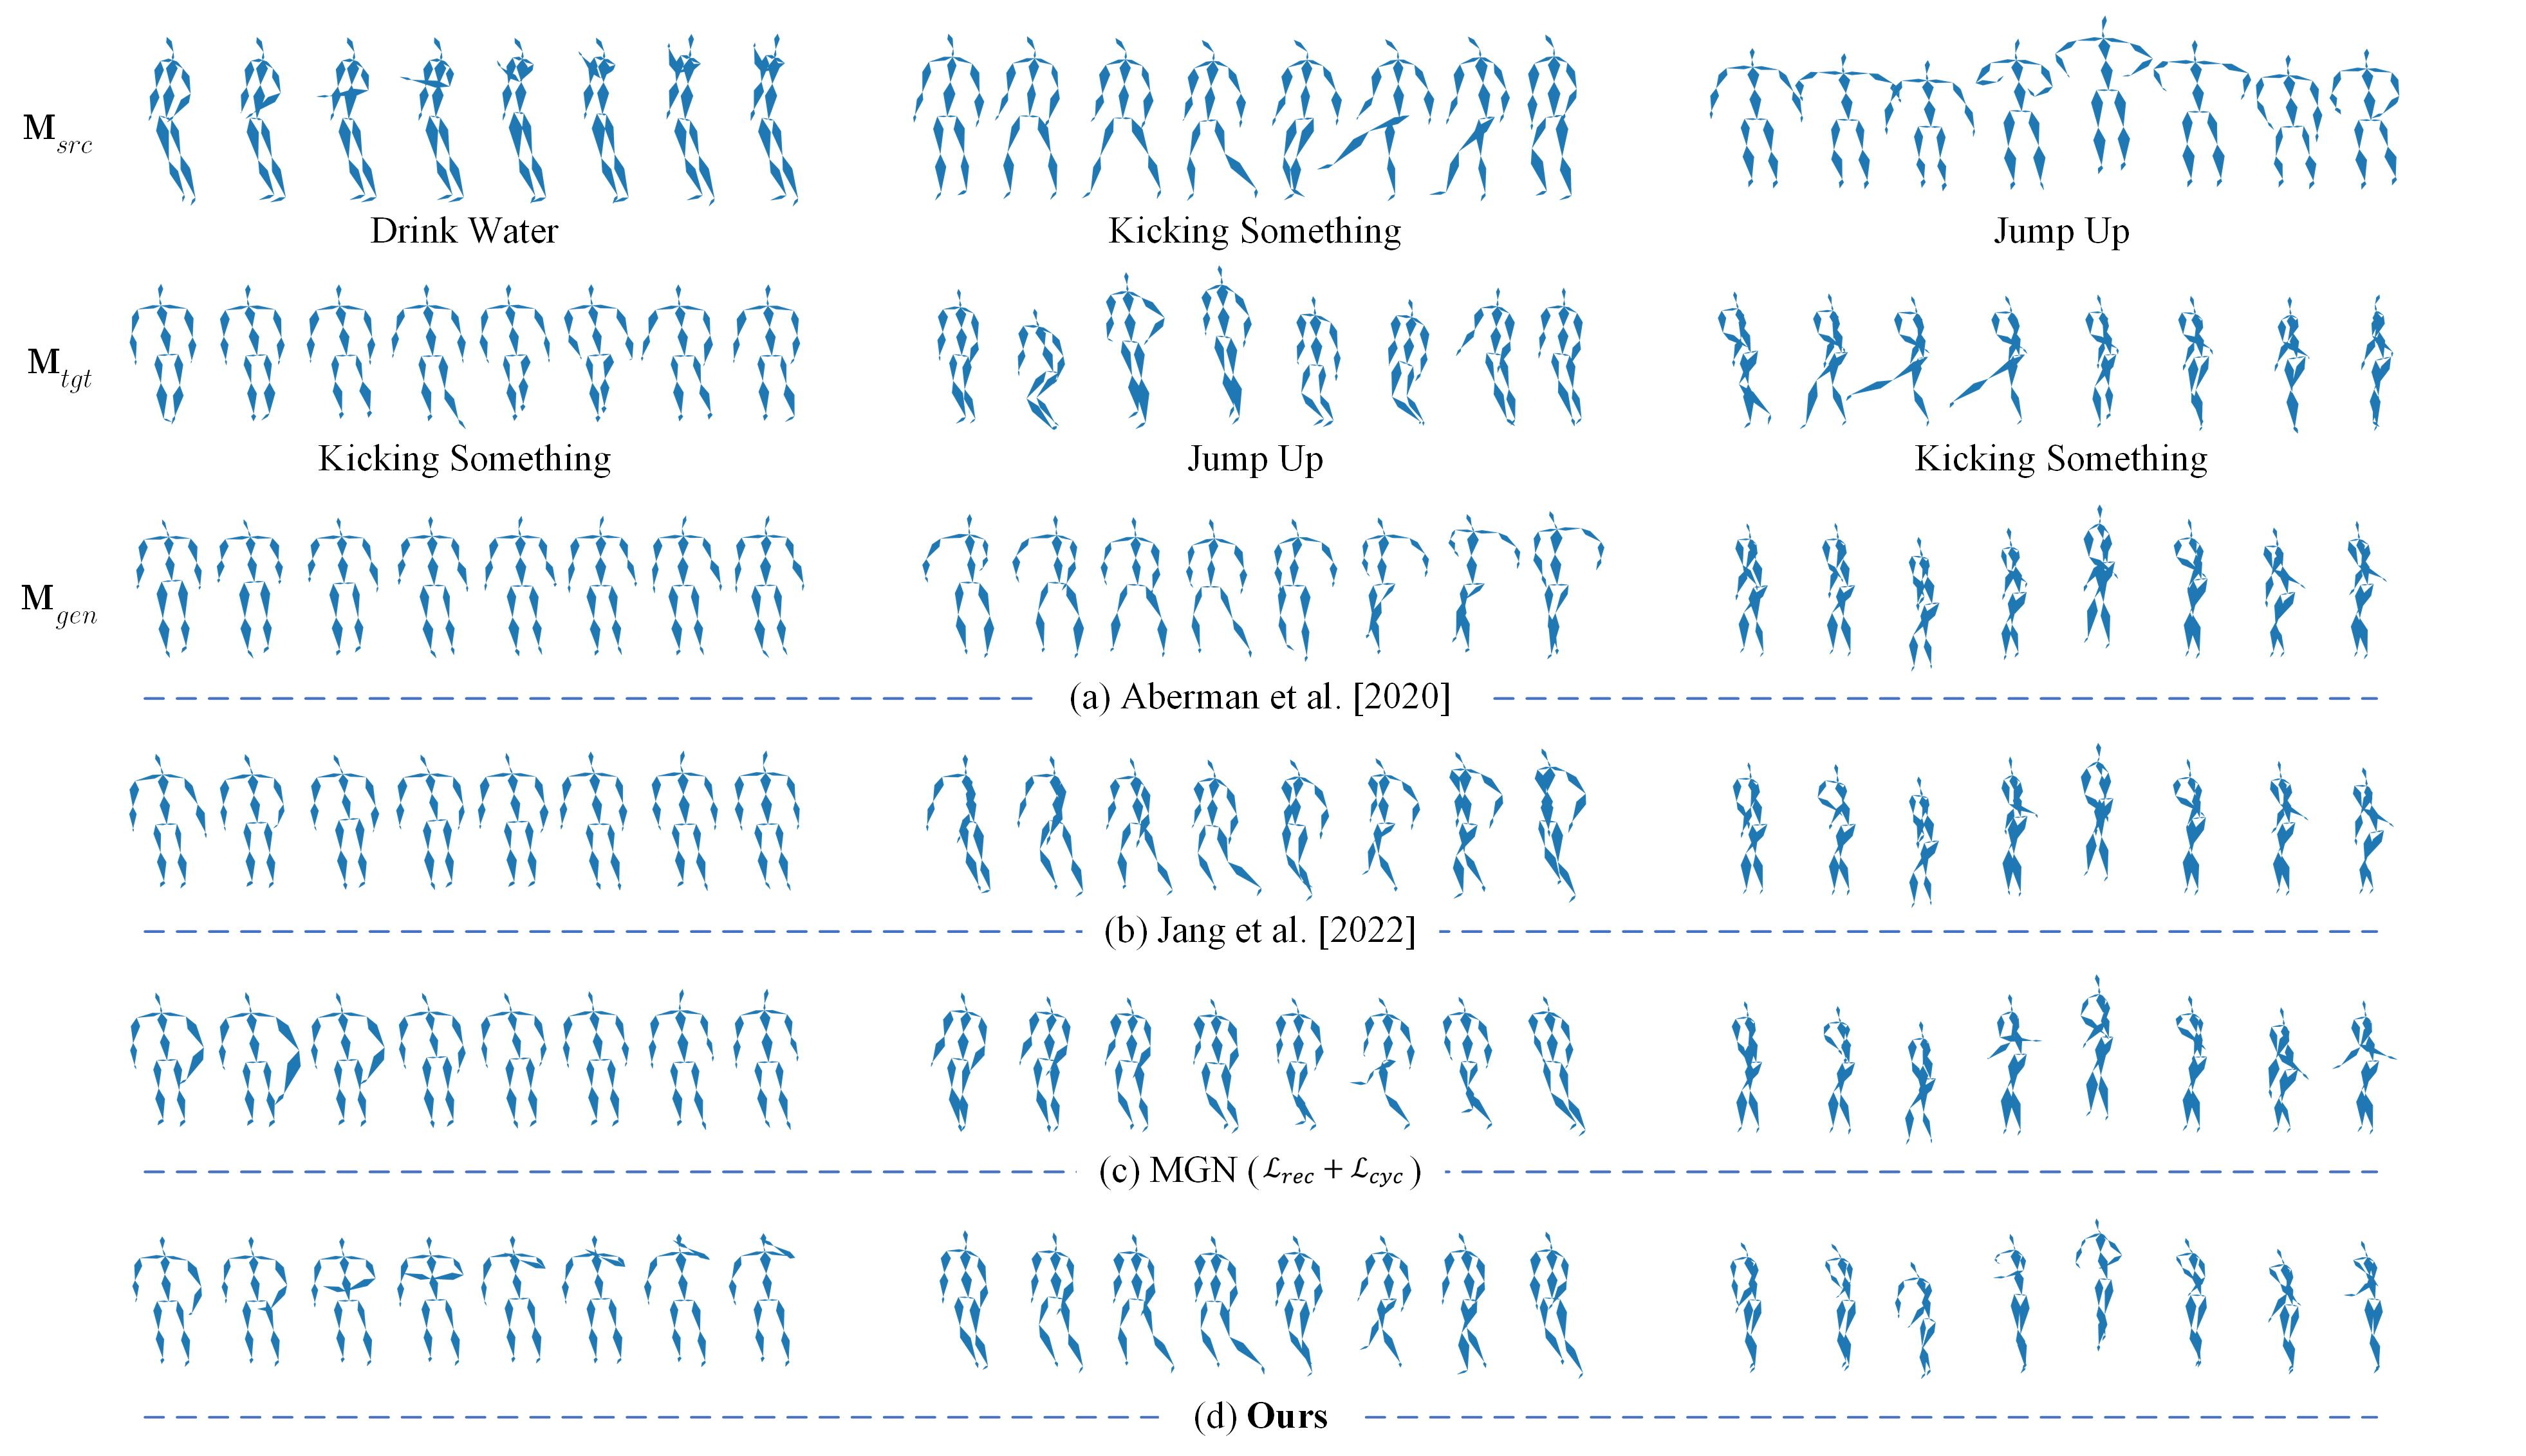
\includegraphics[width=0.8\linewidth]{figures/Fig6.jpg}

   \caption{Comparison results. We used four methods to generate hand action (“Drinking Water”), leg action (“Kicking Something”), and whole-body action (“Jump up”).}
   \label{fig:6}
\end{figure*}

Figure. \ref{fig:6} shows the actions generated by the four methods: (a) the actions generated by Aberman's method, (b) the actions generated by Motion Puzzle, (c) the actions generated by MGN ($\mathcal{L}_{trip}$), and (d) the actions generated by our method.  
Compared to other methods, our method is optimal in generating hand action (“Drinking Water”), leg action (“Kicking Something”), and whole-body action (“Jump up”). 
In (a), (b), and (c), the “Drink Water” (first column) contains only the body morphology of the target action but not the hand moves of the source action. 
The “kicking Something” (second column) and “Jump up” (third column) combine the category features of the source action and the morphology features of the target action very well, but the hand moves are very raw.
Our method generates more natural and coordinated actions, both in terms of the moves of the parts and the overall morphology.

To fully demonstrate that UMN is effective, we sampled 1\% from $\mathcal{M}_{\hat{train}}$ and generated actions using MGN and MGN+UMN, respectively. Then, it is tested according to the action recognition experiment (sec. \ref{sec:motion recognition}). 
Table \ref{tab:4} shows that the average recognition accuracy is 81.48\% for MGN+UMN and 64.96\% for MGN. The results demonstrate that the UMN is effective.

\begin{table}
  \centering
  % \begin{tabular}{@{}lc@{}}
  \resizebox{1\columnwidth}{!}{
  \begin{tabular}{lcccccc}
    \toprule
    & A0 &  A1 & A2 & A3 & A4 & A5  \\
    \midrule
    MGN($\mathcal{L}_{total}$)& 58.29 & 62.72 & 74.62 & 57.32 & 67.88 & 68.91 \\
    MGN($\mathcal{L}_{total}$)+UMN& 84.09 & 79.54 & 78.14 & 81.30 & 82.33 & 83.49 \\
    \bottomrule
  \end{tabular}}
  \caption{Comparison of Top-1 accuracy of MGN($\mathcal{L}_{total}$) and MGN($\mathcal{L}_{total}$)+UMN. Sampling 1\% from $\mathcal{M}_{\hat{train}}$ for action generation.}
  \label{tab:4}
\end{table}


\section{Conclusion}

In this paper, we propose a novel generative network called AGN by introducing active learning. 
AGN can generate many new actions by means of motion transfer with only one or a few samples. 
The AGN consists of the MGN and the UMN. 
The MGN is able to implicitly learn the skeletal morphology of the target action while preserving the category features of the source action. 
The UMN utilizes uncertainty-inspired learning in active learning to provide an uncertainty score for the generation process and thus guides the MGN to improve the quality of the generation. 
AGN showed the best performance compared to the existing methods.FMD is 2.67, and Accuracy is 92.18\%. 
{
    \small
    \bibliographystyle{ieeenat_fullname}
    \bibliography{main}
}

\end{document}
